\documentclass[a4paper,10pt]{article}
\usepackage[left=1.5cm,right=1.5cm,top=1.5cm,bottom=1.5cm]{geometry}
\usepackage{graphicx}
\usepackage{parskip}
\usepackage{enumitem}
\usepackage{titlesec}
\usepackage{multicol}
\usepackage{fontawesome5}
\usepackage{helvet}
\usepackage{xcolor}
\usepackage[skins]{tcolorbox}
\renewcommand{\familydefault}{\sfdefault}

% Couleurs modernes
\definecolor{accentcolor}{RGB}{44,62,80}
\definecolor{secondarycolor}{RGB}{52,152,219}

% Ajustement des espacements
\setlength{\parskip}{4pt}
\setlength{\itemsep}{2pt}

% Titres des sections avec style moderne
\titleformat{\section}{\color{accentcolor}\large\bfseries\uppercase}{}{0em}{}[\titlerule]

% Style pour les compétences
\newtcolorbox{skillbox}{colback=white, colframe=secondarycolor!20, arc=3pt, boxsep=3pt, left=4pt, right=4pt}

\begin{document}

% --- En-tête amélioré ---
\begin{minipage}[t]{0.18\textwidth}
  \vspace{0pt}
  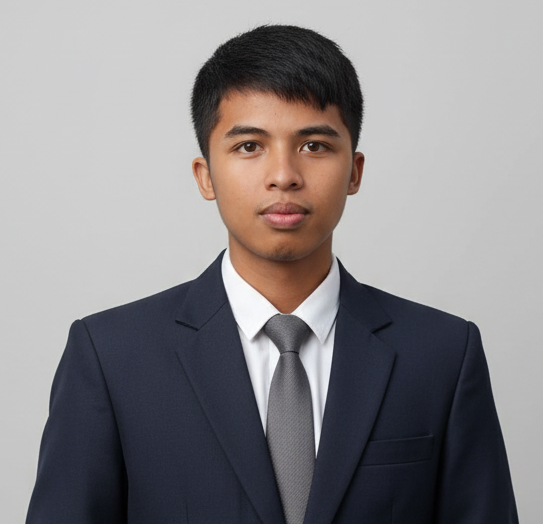
\includegraphics[width=\linewidth]{rajoCv.png}
\end{minipage}
\hfill
\begin{minipage}[t]{0.78\textwidth}
  {\Huge \textbf{\color{accentcolor} Rakotonavalona Rajo Lalaina}}\\[4pt]
  {\large \color{secondarycolor}Étudiant en Informatique – \textbf{Data Analyst Junior}}\\[8pt]
  \faIcon{map-marker-alt}\ \textcolor{accentcolor}{Antananarivo, Madagascar} \hfill
  \faIcon{envelope}\ \textcolor{accentcolor}{valkely02@gmail.com} \\[3pt]
  \faIcon{phone}\ \textcolor{accentcolor}{+261 38 98 826 79} \hfill
  \faIcon{linkedin}\ \textcolor{accentcolor}{linkedin.com/in/rajo} \\[3pt]
  \faIcon{github}\ \textcolor{accentcolor}{github.com/Naval0506}
\end{minipage}

\vspace{0.4cm}
\hrule height1.5pt
\vspace{0.4cm}

% --- Deux colonnes principales ---
\begin{minipage}[t]{0.38\textwidth}

\section*{Profil}
Étudiant passionné par l'analyse et la visualisation de données, je conçois des solutions exploitant Python, SQL et des outils BI pour transformer les données en insights exploitables. Mon objectif : participer à des projets concrets combinant technologie et impact réel.

\section*{Compétences}
\begin{skillbox}
\textbf{Analyse} : nettoyage, exploration, visualisation\\
\textbf{Langages} : Python, SQL, R\\
\textbf{Outils} : Power BI, Tableau, Excel, Jupyter\\
\textbf{ML} : régression, classification, détection d'anomalies\\
\textbf{BDD} : MySQL, PostgreSQL\\
\textbf{Soft skills} : rigueur, autonomie, curiosité
\end{skillbox}

\section*{Formation}
\textbf{Licence en Informatique (en cours)}\\
Université INSI — 2024–2025\\[4pt]
\textbf{Certifications}\\
Google Cloud Skill Boost – Data Analytics

\section*{Langues}
\begin{itemize}[leftmargin=*, label={}]
  \item \textbf{Français} : intermédiaire
  \item \textbf{Anglais} : moyen (technique)
  \item \textbf{Malagasy} : langue maternelle
\end{itemize}

\end{minipage}
\hfill
\begin{minipage}[t]{0.58\textwidth}

\section*{Projets}
\begin{itemize}[leftmargin=*, label={\color{secondarycolor}\scriptsize\faIcon{caret-right}}]
  \item \textbf{Détection de fraudes bancaires (2025)}\\
  \textit{Python, Colab, ML}\\
  Modèles supervisés (régression logistique, forêt aléatoire) pour identifier les transactions suspectes. Interface web de test et enregistrement des prédictions.
  \vspace{4pt}
  
  \item \textbf{Analyse d'habitudes d'achat (2025)}\\
  \textit{Power BI, Python}\\
  Segmentation de clients, tableaux de bord interactifs et recommandations IA pour plateforme e-commerce malgache.
  \vspace{4pt}
  
  \item \textbf{Prédiction du prix des maisons (2024)}\\
  \textit{Ames Housing – ML}\\
  Nettoyage, normalisation et modélisation par régression (Random Forest, Linear) pour estimer les prix immobiliers.
  \vspace{4pt}
  
  \item \textbf{Gestion d'emploi du temps (2024–2025)}\\
  \textit{Symfony, MySQL}\\
  Application web pour planifier et visualiser les sessions de cours selon la semaine et la classe.
\end{itemize}

\section*{Centres d'intérêt}
\begin{itemize}[leftmargin=*, label={\color{secondarycolor}\scriptsize\faIcon{star}}]
  \item Veille technologique (IA, Data Science)
  \item Participation à des hackathons
  \item Développement de projets open source
\end{itemize}

\end{minipage}

\end{document}